\documentclass[12pt,a4paper]{article}
\usepackage{graphicx,textcomp}
\usepackage{natbib}
\usepackage{setspace}
\usepackage{fullpage}
\usepackage{color}
\usepackage[reqno]{amsmath}
\usepackage{amsthm}
\usepackage{fancyvrb}
\usepackage{amssymb,enumerate}
\usepackage[all]{xy}
\usepackage{endnotes}
\usepackage{lscape}
\newtheorem{com}{Comment}
\usepackage{float}
\usepackage{hyperref}
\newtheorem{lem} {Lemma}
\newtheorem{prop}{Proposition}
\newtheorem{thm}{Theorem}
\newtheorem{defn}{Definition}
\newtheorem{cor}{Corollary}
\newtheorem{obs}{Observation}
\usepackage[compact]{titlesec}
\usepackage{dcolumn}
\usepackage{tikz}
\usetikzlibrary{arrows}
\usepackage{multirow}
\usepackage{xcolor}
\usepackage{adjustbox}
\newcolumntype{.}{D{.}{.}{-1}}
\newcolumntype{d}[1]{D{.}{.}{#1}}
\definecolor{light-gray}{gray}{0.65}
\usepackage{url}
\usepackage{listings}
\usepackage{color}

\definecolor{codegreen}{rgb}{0,0.6,0}
\definecolor{codegray}{rgb}{0.5,0.5,0.5}
\definecolor{codepurple}{rgb}{0.58,0,0.82}
\definecolor{backcolour}{rgb}{0.95,0.95,0.92}

\lstdefinestyle{mystyle}{
	backgroundcolor=\color{backcolour},   
	commentstyle=\color{codegreen},
	keywordstyle=\color{magenta},
	numberstyle=\tiny\color{codegray},
	stringstyle=\color{codepurple},
	basicstyle=\footnotesize,
	breakatwhitespace=false,         
	breaklines=true,                 
	captionpos=b,                    
	keepspaces=true,                 
	numbers=left,                    
	numbersep=5pt,                  
	showspaces=false,                
	showstringspaces=false,
	showtabs=false,                  
	tabsize=2
}
\lstset{style=mystyle}
\newcommand{\Sref}[1]{Section~\ref{#1}}
\newtheorem{hyp}{Hypothesis}

\title{Predicting House Prices}
\date{Conor, Linette, Lucas, Minh}
\author{Quantitative Methods 1 (Tutorial)}

\begin{document}

\maketitle

\section{The intuition behind variable selection}

	\noindent To predict the Adjusted Sale Price of houses, we considered three major factors:
	
	\begin{itemize}
		\item the neighbourhood;
		\item the size of the house; and
		\item the quality of the construction. \\
	\end{itemize}
	
	\noindent Figure 1 below summarizes the variables we selected to represent each of those characteristics and their relationship.
	
		\lstinputlisting[language=R, firstline=42, lastline=42]{model_template.R} 	
	
	\begin{figure}[H]
		\centering
		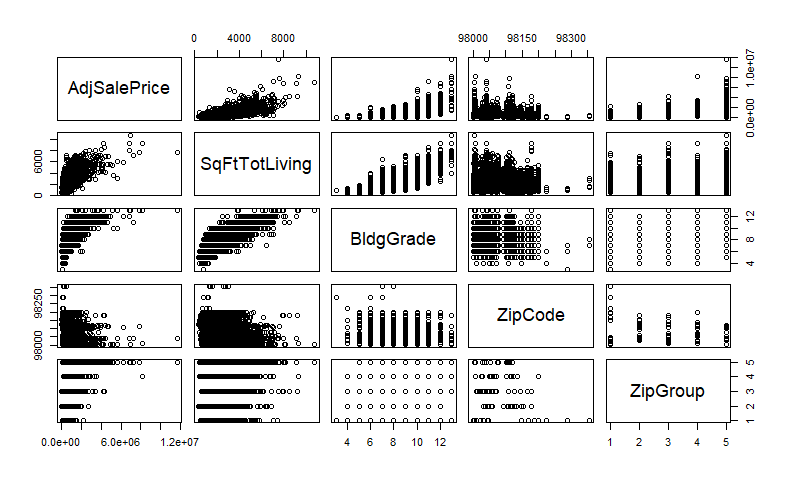
\includegraphics[width=1\linewidth]{AdjSalePrice_pairs}
		\caption{Associations of \texttt{AdjSalePrice} with \texttt{SqFtTotLiving}, \texttt{BldgGrade}, and \texttt{ZipCode}}
		\label{fig:adjsalepricepairs}
	\end{figure}
		
	\noindent \texttt{ZipCode} represents \textbf{neighborhood}. We grouped zip codes based on house prices in the variable \texttt{ZipGroup} to reflect the socioeconomic profile of each neighborhood. \\
	
		\lstinputlisting[language=R, firstline=18, lastline=27]{model_template.R} 
	
	\noindent \texttt{SqFtTotLiving} represents the \textbf{size of the house}. We avoided adding to the model the variables \texttt{SqFtLot}, \texttt{SqFtFinBasement}, \texttt{NbrLivingUnits} \texttt{Bathrooms}, and \texttt{Bedrooms} because they are also related to the size of the construction. That decision allowed us to reach a more \textbf{parsimonious} model, preventing us from loosing degrees of freedom and from incurring in issues related to \textbf{collinearity}. The risk of collinearity among those variables is visible in Figure 2 below: \\
	
		\lstinputlisting[language=R, firstline=43, lastline=43]{model_template.R} 
	
	\begin{figure}[H]
		\centering
		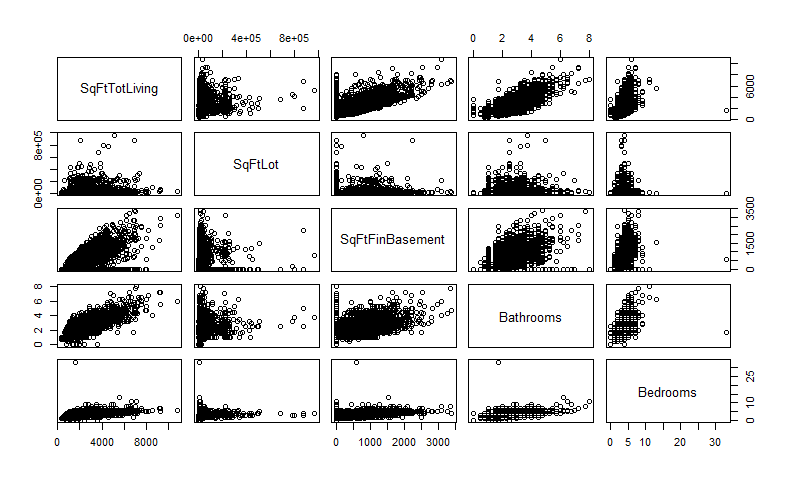
\includegraphics[width=1\linewidth]{SqFtTotLiving_pairs}
		\caption{Risk of collinearity among \texttt{SqFtLot}, \texttt{SqFtFinBasement}, \texttt{Bathrooms}, and \texttt{Bedrooms}}
		\label{fig:sqfttotlivingpairs}
	\end{figure}
		
	\noindent Lastly, \texttt{BldgGrade} represents the \textbf{quality of the construction}. For the same reasons stated above (parsimony, preventing the loss of degrees of freedom, and avoiding collinearity issues), we decided not to add \texttt{YrBuilt}, \texttt{YrRenovated}, and \texttt{NewConstruction}, which are also related to the quality of the construction. \\
	
\vspace{.5cm}

\section{The intuition behind the interaction effect}

	To complete the model, we added an interaction effect between \texttt{ZipGroup} and \texttt{SqFtTotLiving}. The interaction reflects the idea that each additional square foot in the building will affect house prices differently depending on the neighborhood. As a consequence, the slope of \texttt{SqFtTotLiving} on \texttt{AdjSalePrice} in expensive neighborhoods will be steeper than in popular ones (as can be seen in Figure 3).

		\lstinputlisting[language=R, firstline=44, lastline=46]{model_template.R}

		\begin{figure}[H]
			\centering
			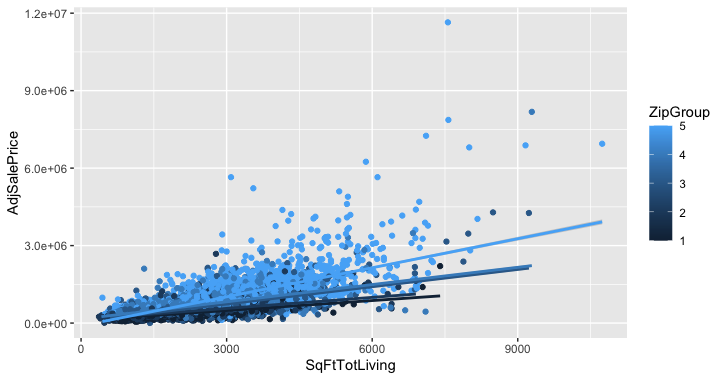
\includegraphics[width=1\linewidth]{Rplot}
			\caption{The effect of \texttt{SqFtTotLiving} on \texttt{AdjSalePrice} by \texttt{ZipGroup}}
			\label{fig:rplot}
		\end{figure}

\vspace{.5cm}

\section{Final model}

The effects of \texttt{SqFtTotLiving}, \texttt{BldgGrade}, \texttt{as.factor(ZipGroup)}, and \texttt{SqFtTotLiving:ZipGroup} on \texttt{AdjSalePrice}

	\lstinputlisting[language=R, firstline=30, lastline=36]{model_template.R} 

\begin{table}[H] \centering 
	\caption{The effects of \texttt{SqFtTotLiving}, \texttt{BldgGrade}, \texttt{as.factor(ZipGroup)}, and \texttt{SqFtTotLiving:ZipGroup} on \texttt{AdjSalePrice}} 
	\label{}
	\begin{adjustbox}{width=1\textwidth}
	\begin{tabular}{@{\extracolsep{5pt}}lcccc} 
		\\[-1.8ex]\hline 
		\hline \\[-1.8ex] 
		& \multicolumn{4}{c}{\textit{Dependent variable:}} \\ 
		\cline{2-5} 
		\\[-1.8ex] & \multicolumn{4}{c}{AdjSalePrice} \\ 
		\\[-1.8ex] & (1) & (2) & (3) & (4)\\ 
		\hline \\[-1.8ex] 
		SqFtTotLiving & 294.357$^{***}$ &  &  & $-$45.169$^{***}$ \\ 
		& (2.132) &  &  & (5.890) \\ 
		& & & & \\ 
		BldgGrade &  & 221,513.500$^{***}$ &  & 74,339.440$^{***}$ \\ 
		&  & (1,695.289) &  & (2,324.481) \\ 
		& & & & \\ 
		ZipGroup &  &  & 134,825.800$^{***}$ &  \\ 
		&  &  & (1,767.656) &  \\ 
		& & & & \\ 
		as.factor(ZipGroup)2 &  &  &  & $-$60,600.140$^{***}$ \\ 
		&  &  &  & (6,261.020) \\ 
		& & & & \\ 
		as.factor(ZipGroup)3 &  &  &  & $-$112,855.500$^{***}$ \\ 
		&  &  &  & (7,949.155) \\ 
		& & & & \\ 
		as.factor(ZipGroup)4 &  &  &  & $-$168,392.000$^{***}$ \\ 
		&  &  &  & (9,795.236) \\ 
		& & & & \\ 
		as.factor(ZipGroup)5 &  &  &  & $-$257,812.900$^{***}$ \\ 
		&  &  &  & (13,626.880) \\ 
		& & & & \\ 
		SqFtTotLiving:ZipGroup &  &  &  & 64.755$^{***}$ \\ 
		&  &  &  & (1.442) \\ 
		& & & & \\ 
		Constant & $-$47,126.100$^{***}$ & $-$1,136,579.000$^{***}$ & 138,024.100$^{***}$ & $-$232,072.400$^{***}$ \\ 
		& (4,843.068) & (13,173.570) & (6,085.377) & (15,604.750) \\ 
		& & & & \\ 
		\hline \\[-1.8ex] 
		Observations & 20,340 & 20,340 & 20,340 & 20,340 \\ 
		R$^{2}$ & 0.484 & 0.456 & 0.222 & 0.622 \\ 
		Adjusted R$^{2}$ & 0.484 & 0.456 & 0.222 & 0.621 \\
		Residual Std. Error & 278,257.400 & 285,528.100 & 341,480.700 & 238,266.300 \\ 
		& (df = 20338) & (df = 20338) & (df = 20338) & (df = 20332) \\
		F Statistic & 19,053.750$^{***}$ & 17,073.130$^{***}$ & 5,817.690$^{***}$ & 4,770.375$^{***}$ \\ 
		& (df = 1; 20338) & (df = 1; 20338) & (df = 1; 20338) & (df = 7; 20332) \\
		\hline 
		\hline \\[-1.8ex] 
		\textit{Note:}  & \multicolumn{4}{r}{$^{*}$p$<$0.1; $^{**}$p$<$0.05; $^{***}$p$<$0.01} \\ 
	\end{tabular}
	\end{adjustbox}
\end{table} 

\end{document}
